\documentclass[conference]{IEEEtran}

\usepackage{graphicx}
\usepackage{xcolor}
\usepackage{amsmath}
\usepackage{amssymb}
\usepackage{amsthm}
\usepackage{booktabs}
\usepackage{algorithm}
\usepackage{algpseudocode}
\usepackage{enumitem}

\newtheorem{theorem}{Theorem}
\newtheorem{remark}{Remark}

\usepackage[
    colorlinks=true,
    linkcolor=black,
    citecolor=darkgray,
    urlcolor=blue,
    bookmarks=true,
    bookmarksnumbered=true,
    unicode=true
]{hyperref}

\hypersetup{
    pdftitle={Near-Field Secure ISAC with STAR-RIS for Spoofing-Resilient LEO Satellite Navigation in 6G NTN},
    pdfauthor={Author Name},
    pdfsubject={Satellite Communications},
    pdfkeywords={LEO, ISAC, STAR-RIS, near-field, physical layer security, spoofing}
}

\title{Near-Field Secure ISAC with STAR-RIS for Spoofing-Resilient LEO Satellite Navigation in 6G Non-Terrestrial Networks}

\author{
\IEEEauthorblockN{Author Name}
\IEEEauthorblockA{Department of Electrical Engineering\\
Email: author@university.edu}
}

\begin{document}

\maketitle

\begin{abstract}
We propose a near-field integrated sensing and communications (ISAC) framework for spoofing-resilient low-Earth-orbit (LEO) satellite navigation in 6G non-terrestrial networks (NTN), assisted by a simultaneously transmitting and reflecting reconfigurable intelligent surface (STAR-RIS). A LEO satellite with a large-scale array broadcasts navigation signals to ground users located on both sides of a ground-deployed STAR-RIS, in the presence of an active spoofer injecting counterfeit navigation signals. Since the spoofer is non-cooperative, a ground ISAC anchor exploits near-field spherical-wave propagation to localize and track it from echo signals via an extended Kalman filter (EKF), without pilot cooperation. Based on the reconstructed spoofer channel, we jointly optimize the satellite's active beamforming and the STAR-RIS transmission/reflection coefficients to maximize the sum secrecy rate, subject to a Cram\'er--Rao bound (CRB) constraint on the spoofer localization accuracy, the satellite power budget, and the STAR-RIS energy conservation constraint. The resulting non-convex problem is solved by an alternating optimization (AO) algorithm combining successive convex approximation (SCA) and a penalty-based treatment of the energy constraint. Simulation results show that: 1) the proposed design achieves a sum secrecy rate of up to 17\,bps/Hz, consistently outperforming a conventional reflection-only RIS, a random-phase STAR-RIS (near zero), and a blocked direct link; 2) the AO algorithm converges within a few iterations; and 3) the near-field model yields a meter-level spoofer range CRB ($\approx 0.84$\,m at 50\,m) and an EKF tracking RMSE of $\approx 0.36$\,m, whereas the far-field model renders the range fundamentally unobservable.
\end{abstract}

\begin{IEEEkeywords}
6G, non-terrestrial networks, LEO satellite navigation, integrated sensing and communications (ISAC), STAR-RIS, near field, physical layer security, spoofing.
\end{IEEEkeywords}

\section{Introduction}\label{sec:intro}

Low-Earth-orbit (LEO) satellite constellations are a key pillar of 6G non-terrestrial networks (NTN), providing global positioning, navigation, and timing (PNT) as well as broadband connectivity. However, the broadcast nature and long propagation distance of satellite-to-ground links make LEO navigation signals highly vulnerable to \emph{spoofing} attacks, in which an adversary injects counterfeit signals to mislead the position estimation of legitimate users.

Physical layer security (PLS) techniques, particularly beamforming-based secrecy enhancement, have been extensively studied for terrestrial and UAV networks~\cite{zeng2016uav,wu2020ris}. In~\cite{zhao2025nearfield}, a near-field ISAC framework was proposed for secure UAV networks, where artificial noise (AN) is used for both jamming and sensing, and the eavesdropper's 3D velocity is estimated from near-field Doppler observations with an extended Kalman filter (EKF); near-field velocity sensing and predictive beamforming were further developed in~\cite{wang2025velocity}. STAR-RIS has been shown to provide full-space $360^\circ$ coverage by simultaneously transmitting and reflecting incident signals~\cite{zhao2022starris,mu2022starris,xu2021starris}, and its active variant can compensate the multiplicative path loss of cascaded channels~\cite{zhao2025aerial,zhang2023activeris}. The dual-functional ISAC paradigm itself is surveyed in~\cite{liu2022isac}, and near-field ISAC beamforming for target detection was studied in~\cite{galappaththige2024nearfield,cao2024nearfield}.

Nevertheless, three gaps remain open:
\begin{enumerate}[leftmargin=1.5em]
    \item Existing near-field secure ISAC designs focus on terrestrial/UAV scenarios with short link distances; the LEO-to-ground geometry with strong orbital Doppler has not been addressed.
    \item Existing STAR-RIS designs target sum-rate maximization and do not consider spoofing threats or sensing-aided security.
    \item Spoofing-resilient navigation, which requires both \emph{detection/localization of the attacker} and \emph{protective beamforming}, has not been jointly treated with STAR-RIS in near field.
\end{enumerate}

Motivated by the above, this project develops a near-field secure ISAC framework for spoofing-resilient LEO navigation aided by a STAR-RIS. The contributions are summarized as follows:
\begin{itemize}[leftmargin=1.5em]
    \item \textbf{New system model:} To the best of our knowledge, one of the first combinations of near-field propagation, STAR-RIS, and ISAC for an LEO-NTN navigation scenario under an active spoofing attack. In contrast to~\cite{zhao2025nearfield}, which considers a passive eavesdropper in a terrestrial UAV scenario, we address an \emph{active injecting spoofer} in the LEO-NTN geometry and exploit its \emph{sensed} location in the secrecy design. A hybrid far-field/near-field cascaded channel model is developed: the satellite-to-STAR-RIS link follows far-field LoS propagation with orbital Doppler, while the STAR-RIS-to-user and STAR-RIS-to-spoofer links operate in the near-field (Fresnel) region.
    \item \textbf{New CRB analysis:} A Cram\'er--Rao bound for spoofer 3D localization over the STAR-RIS cascaded near-field channel is derived and used as an explicit sensing-accuracy constraint in the design.
    \item \textbf{New joint optimization algorithm:} An AO algorithm jointly designs the satellite active beamforming and the STAR-RIS transmission/reflection coefficients to maximize the sum secrecy rate under power, energy-conservation, and CRB constraints, tackled via SCA with a penalty-based treatment of the STAR-RIS energy-conservation constraint, with convergence and complexity analysis.
\end{itemize}

\emph{Organization:} Section~\ref{sec:model} presents the system model. Section~\ref{sec:problem} formulates the optimization problem and Section~\ref{sec:alg} develops the AO algorithm. Section~\ref{sec:sim} lists the simulation parameters, Section~\ref{sec:results} reports the numerical results, and Section~\ref{sec:concl} concludes the paper.

\section{System Model}\label{sec:model}

\subsection{Scenario}
As illustrated in Fig.~\ref{fig:sysmodel}, a LEO satellite (S) equipped with a uniform planar array (UPA) of $N = N_x \times N_y$ antennas transmits navigation/communication signals to $K$ legitimate ground users (GUs) with the aid of a ground-deployed STAR-RIS with $M$ elements.

\begin{figure}[t]
\centering
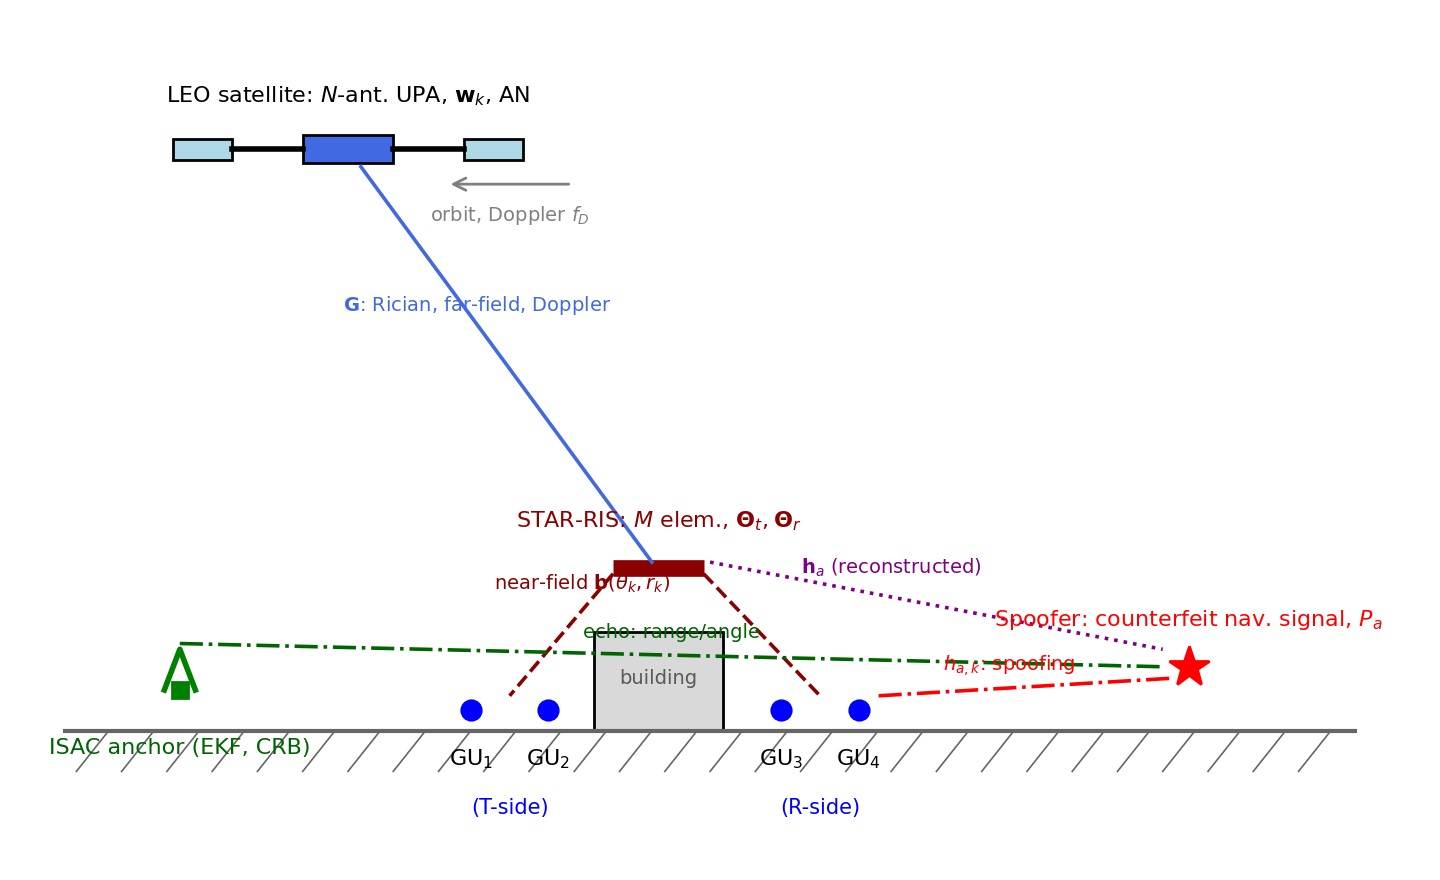
\includegraphics[width=\columnwidth]{figs/fig_system_model.png}
\caption{System model: a LEO satellite serves ground users on both sides of a ground-deployed STAR-RIS; a ground ISAC anchor localizes the active spoofer via near-field echoes.}
\label{fig:sysmodel}
\end{figure} The GUs are partitioned into a transmission-side set $\mathcal{K}_t$ ($|\mathcal{K}_t| = K_t$) and a reflection-side set $\mathcal{K}_r$ ($|\mathcal{K}_r| = K_r$), with $K = K_t + K_r$. An active spoofer (A), located in the reflection half-space, injects a counterfeit navigation signal $s_a(t)$ to mislead the GUs' position estimation. The spoofer is non-cooperative and its channel state information (CSI) is unknown a priori; a ground ISAC anchor node senses the spoofer and provides real-time state estimates (Section~\ref{sec:sensing}).

\subsection{Channel Model}
\subsubsection{Satellite-to-STAR-RIS link (far-field with orbital Doppler)}
Given the large link distance ($\sim$500--1200\,km), the S-to-RIS link is modeled as far-field LoS:
\begin{equation}\label{eq:gsr}
    \mathbf{G} = \sqrt{\beta_{\mathrm{SR}}}\, e^{j 2\pi f_D t} \left( \sqrt{\frac{\kappa}{1+\kappa}}\, \mathbf{a}_M(\vartheta_{\mathrm{SR}})\, \mathbf{a}_N^H(\theta_{\mathrm{SR}}, \phi_{\mathrm{SR}}) + \sqrt{\frac{1}{1+\kappa}}\, \widetilde{\mathbf{G}} \right) \in \mathbb{C}^{M \times N},
\end{equation}
where $\beta_{\mathrm{SR}} = \left(\frac{\lambda}{4\pi d_{\mathrm{SR}}}\right)^2 G_s G_r$ is the large-scale path gain, $f_D$ is the orbital Doppler shift induced by the satellite motion, $\mathbf{a}_N \in \mathbb{C}^{N}$ and $\mathbf{a}_M \in \mathbb{C}^{M}$ are the far-field steering vectors of the satellite array and the STAR-RIS (departure/arrival), $\kappa$ is the Rician factor of the satellite link, and $\widetilde{\mathbf{G}}$ is the scattered (NLoS) component with i.i.d.\ $\mathcal{CN}(0,1)$ entries. The Rician component is essential: a purely LoS rank-one $\mathbf{G}$ would make all cascaded user channels collinear, rendering satellite-side beamforming unable to separate the users.

\subsubsection{STAR-RIS-to-node links (near-field)}
The STAR-RIS aperture is large relative to the RIS-to-user distances, so the GUs and the spoofer lie in its near-field region. The near-field channel vector from the RIS to a node at distance $r$ and angle $\theta$ is
\begin{equation}\label{eq:nfsteer}
    [\mathbf{b}(\theta, r)]_m = \frac{1}{\sqrt{M}} e^{-j\frac{2\pi}{\lambda}(r_m - r)}, \quad r_m = \sqrt{r^2 + \delta_m^2 d^2 - 2 r \delta_m d \sin\theta},
\end{equation}
where $d$ is the element spacing and $\delta_m = \frac{2m - M - 1}{2}$, $m = 1,\dots,M$. Unlike the far-field model, the phase depends on both angle and distance, enabling \emph{distance-angle} resolution.

The overall cascaded channel from the satellite to GU $k \in \mathcal{K}_\chi$, $\chi \in \{t, r\}$, is
\begin{equation}\label{eq:cascade}
    \mathbf{h}_k^H = \sqrt{\beta_k}\, \mathbf{b}^H(\theta_k, r_k)\, \boldsymbol{\Theta}_\chi\, \mathbf{G},
\end{equation}
where $\boldsymbol{\Theta}_t = \mathrm{diag}(\boldsymbol{\theta}_t)$ and $\boldsymbol{\Theta}_r = \mathrm{diag}(\boldsymbol{\theta}_r)$ are the STAR-RIS transmission and reflection coefficient matrices, with $[\boldsymbol{\theta}_\chi]_m = \beta_{\chi,m} e^{j\varphi_{\chi,m}}$, subject to the energy conservation constraint
\begin{equation}\label{eq:unity}
    \beta_{t,m}^2 + \beta_{r,m}^2 = 1, \quad \varphi_{t,m},\varphi_{r,m} \in [0, 2\pi), \ \forall m.
\end{equation}
Similarly, the satellite-to-spoofer cascaded channel is $\mathbf{h}_a^H = \sqrt{\beta_a}\, \mathbf{b}^H(\theta_a, r_a)\, \boldsymbol{\Theta}_r\, \mathbf{G}$.

\subsubsection{Spoofer-to-user link}
The spoofer broadcasts its counterfeit signal to the GUs over channel $h_{a,k} = \sqrt{\beta_{a,k}}\, e^{-j 2\pi \tau_{a,k} f_c}$, where $\tau_{a,k}$ is the propagation delay (the key quantity manipulated in a navigation spoofing attack).

\subsection{Signal Model and Secrecy Rate}
The satellite transmits $\mathbf{x} = \sum_{k=1}^{K} \mathbf{w}_k s_k + \mathbf{z}$, where $\mathbf{w}_k \in \mathbb{C}^N$ is the beamformer for GU $k$, $s_k$ its navigation signal with $\mathbb{E}|s_k|^2 = 1$, and $\mathbf{z} \sim \mathcal{CN}(\mathbf{0}, \mathbf{Z})$ is artificial noise (AN) used for both jamming the spoofer and exciting sensing echoes. The SINR at GU $k$ is
\begin{equation}\label{eq:sinr_u}
    \gamma_k = \frac{|\mathbf{h}_k^H \mathbf{w}_k|^2}{\sum_{j \neq k} |\mathbf{h}_k^H \mathbf{w}_j|^2 + \mathbf{h}_k^H \mathbf{Z} \mathbf{h}_k + P_a |h_{a,k}|^2 + \sigma_k^2},
\end{equation}
where $P_a$ is the spoofer transmit power. The leakage SINR at the spoofer for GU $k$'s signal is
\begin{equation}\label{eq:sinr_a}
    \gamma_{a,k} = \frac{|\mathbf{h}_a^H \mathbf{w}_k|^2}{\sum_{j \neq k} |\mathbf{h}_a^H \mathbf{w}_j|^2 + \mathbf{h}_a^H \mathbf{Z} \mathbf{h}_a + \sigma_a^2}.
\end{equation}
The achievable secrecy rate of GU $k$ against the spoofer is
\begin{equation}\label{eq:secrate}
    R_k^{\mathrm{sec}} = \big[\log_2(1 + \gamma_k) - \log_2(1 + \gamma_{a,k})\big]^+.
\end{equation}

\begin{remark}
Since the spoofer is non-cooperative, $\mathbf{h}_a$ cannot be obtained via pilot-based estimation. Following the sensing-aided paradigm of~\cite{zhao2025nearfield}, $\mathbf{h}_a$ is \emph{reconstructed} from the spoofer's estimated position $(\theta_a, r_a)$ via~\eqref{eq:nfsteer}--\eqref{eq:cascade}.
\end{remark}

\begin{remark}[Why secrecy rate for a spoofing scenario?]
A spoofer is primarily an \emph{injecting} adversary rather than a passive eavesdropper. Our formulation addresses both facets: (i) the spoofing interference $P_a|h_{a,k}|^2$ appears directly in the user SINR~\eqref{eq:sinr_u}, so maximizing the users' rates inherently boosts spoofing resilience; (ii) the secrecy rate~\eqref{eq:secrate} protects the navigation message and its authentication data from being read/relayed by the spoofer (meaconing); (iii) the CRB constraint (Section~\ref{sec:problem}) guarantees that the spoofer itself is accurately localized for subsequent mitigation.
\end{remark}

\subsection{Sensing and Tracking of the Spoofer}\label{sec:sensing}
The ISAC anchor receives echoes of the AN waveform reflected by the spoofer (full-duplex echo reception~\cite{sabharwal2014fullduplex}). Exploiting near-field spherical-wave propagation, the spoofer's 3D velocity is estimated from the variation of the Doppler shift across the spatial domain, and an EKF fuses the predicted and measured states:
\begin{equation}\label{eq:ekf}
    \boldsymbol{\xi}_{a}(t) = [\theta_a, r_a, v_x, v_y, v_z]^T, \qquad \hat{\boldsymbol{\xi}}_{a}(t|t) = \mathrm{EKF}\big(\hat{\boldsymbol{\xi}}_{a}(t|t{-}1),\, \mathbf{y}_{\mathrm{echo}}(t)\big).
\end{equation}
The estimation accuracy is quantified by the CRB of the spoofer parameters $\boldsymbol{\eta} = [\theta_a, r_a]^T$. Given the echo model $\mathbf{y} = \sqrt{P_s}\,\mathbf{b}(\theta_a, r_a) + \mathbf{n}$ with $\mathbf{n} \sim \mathcal{CN}(\mathbf{0}, \sigma^2 \mathbf{I}_M)$ at the anchor, the Fisher information matrix (FIM) is
\begin{equation}\label{eq:fim}
    \mathbf{F} = \frac{2 P_s}{\sigma^2}\, \mathrm{Re}\!\left\{ \mathbf{D}^H \mathbf{D} \right\}, \qquad \mathbf{D} = \left[ \frac{\partial \mathbf{b}}{\partial \theta_a},\ \frac{\partial \mathbf{b}}{\partial r_a} \right],
\end{equation}
and the range CRB is $\mathrm{CRB}_r = [\mathbf{F}^{-1}]_{22}$. Under the far-field approximation, $\partial \mathbf{b}/\partial r_a = \mathbf{0}$, so $\mathbf{F}$ is singular and the range is unobservable --- the key motivation for near-field sensing (cf.\ Section~\ref{sec:results}). The impact of the STAR-RIS phase profile on~\eqref{eq:fim} over the cascaded channel is left to the journal extension.

\subsection{LEO-Specific Considerations}
Compared to the terrestrial baseline~\cite{zhao2025nearfield}, the LEO scenario introduces: (i) time-varying elevation angle and strong orbital Doppler $f_D(t)$ (up to tens of kHz at L/S band), requiring Doppler pre-compensation in~\eqref{eq:gsr}; (ii) large-scale free-space path loss, making the STAR-RIS gain essential; (iii) visibility windows, within which the optimization in Section~\ref{sec:problem} is re-solved per time slot.

\section{Problem Formulation}\label{sec:problem}

We maximize the sum secrecy rate of the legitimate users by jointly optimizing the satellite beamformers $\{\mathbf{w}_k\}$, the AN covariance $\mathbf{Z}$, and the STAR-RIS coefficients $\{\boldsymbol{\theta}_t, \boldsymbol{\theta}_r\}$, subject to the sensing accuracy, power, and STAR-RIS energy constraints:

\begin{subequations}\label{eq:opt}
\begin{align}
\max_{\{\mathbf{w}_k\}, \mathbf{Z}, \boldsymbol{\theta}_t, \boldsymbol{\theta}_r} \quad & \sum_{k=1}^{K} R_k^{\mathrm{sec}} \label{eq:opt_obj}\\
\text{s.t.} \quad & \mathrm{CRB}(\hat{r}_a, \hat{\theta}_a; \mathbf{Z}, \boldsymbol{\Theta}_r) \le \epsilon_{\mathrm{CRB}}, \label{eq:opt_crb}\\
& \sum_{k=1}^{K} \|\mathbf{w}_k\|^2 + \mathrm{Tr}(\mathbf{Z}) \le P_{\max}, \label{eq:opt_pow}\\
& \beta_{t,m}^2 + \beta_{r,m}^2 = 1, \quad \forall m, \label{eq:opt_unity}\\
& R_k^{\mathrm{sec}} \ge R_k^{\min}, \quad \forall k, \label{eq:opt_qos}
\end{align}
\end{subequations}
where~\eqref{eq:opt_crb} guarantees the spoofer localization accuracy, \eqref{eq:opt_pow} is the satellite power budget, \eqref{eq:opt_unity} enforces STAR-RIS energy conservation, and~\eqref{eq:opt_qos} imposes a minimum secrecy rate per user.

Problem~\eqref{eq:opt} is non-convex due to (i) the coupled fractional secrecy-rate objective, (ii) the rank/unity-modulus-type constraints in~\eqref{eq:opt_unity}, and (iii) the bilinear coupling between $\boldsymbol{\Theta}_\chi$ and $\mathbf{w}_k$ in the cascaded channels~\eqref{eq:cascade}.

\section{Proposed Algorithm}\label{sec:alg}

We develop an alternating optimization (AO) algorithm that decouples~\eqref{eq:opt} into three subproblems, solved iteratively until convergence.

\subsection{Satellite Beamforming and AN Design}
Given $(\boldsymbol{\theta}_t, \boldsymbol{\theta}_r)$, the subproblem over $(\{\mathbf{w}_k\}, \mathbf{Z})$ is handled by introducing slack variables for the difference-of-logarithms objective and applying successive convex approximation (SCA) with first-order Taylor expansions of the concave terms at the current iterate, following the framework of~\cite{zhao2025nearfield}. Each SCA step is a convex QCQP/SDP solvable by standard solvers (e.g., CVX/MOSEK).

\subsection{STAR-RIS Coefficient Design}
Given $(\{\mathbf{w}_k\}, \mathbf{Z})$, the coefficients $\boldsymbol{\theta}_t, \boldsymbol{\theta}_r$ are optimized by combining the amplitude and phase of each element into a joint variable as in~\cite{zhao2025aerial}, and relaxing the energy-conservation constraint~\eqref{eq:opt_unity} via a penalty term $\rho \sum_m \big(\beta_{t,m}^2 + \beta_{r,m}^2 - 1\big)^2$ appended to the objective; the penalty weight $\rho$ is increased across iterations (penalty-based method), followed by a projection onto the feasible set of~\eqref{eq:opt_unity}.

\subsection{Overall Algorithm}
\begin{algorithm}[t]
\caption{Proposed AO Algorithm for Problem~\eqref{eq:opt}}
\label{alg:ao}
\begin{algorithmic}[1]
\Require Initial feasible $(\{\mathbf{w}_k^{(0)}\}, \mathbf{Z}^{(0)}, \boldsymbol{\theta}_t^{(0)}, \boldsymbol{\theta}_r^{(0)})$; penalty $\rho^{(0)}$; tolerance $\epsilon$; EKF estimate $\hat{\boldsymbol{\xi}}_a$ from~\eqref{eq:ekf}.
\Repeat
    \State Update $(\{\mathbf{w}_k^{(i)}\}, \mathbf{Z}^{(i)})$ via SCA given $(\boldsymbol{\theta}_t^{(i-1)}, \boldsymbol{\theta}_r^{(i-1)})$;
    \State Update $(\boldsymbol{\theta}_t^{(i)}, \boldsymbol{\theta}_r^{(i)})$ via penalty-based method given $(\{\mathbf{w}_k^{(i)}\}, \mathbf{Z}^{(i)})$;
    \State Increase penalty weight $\rho^{(i)}$; $i \leftarrow i+1$;
\Until{relative increase of~\eqref{eq:opt_obj} $< \epsilon$ and penalty residual $< \epsilon$.}
\Ensure $(\{\mathbf{w}_k^\star\}, \mathbf{Z}^\star, \boldsymbol{\theta}_t^\star, \boldsymbol{\theta}_r^\star)$.
\end{algorithmic}
\end{algorithm}

\begin{theorem}[Convergence]
Algorithm~\ref{alg:ao} generates a non-decreasing sequence of objective values of~\eqref{eq:opt_obj} and converges to a Karush--Kuhn--Tucker (KKT) point of the penalized problem; as $\rho \to \infty$, the solution satisfies~\eqref{eq:opt_unity} and is a KKT point of~\eqref{eq:opt}.
\end{theorem}
\begin{proof}[Proof sketch]
Each SCA subproblem is convex and its solution does not decrease the surrogate objective, which lower-bounds~\eqref{eq:opt_obj}; the penalty subproblem is bounded below and monotonically converges. The boundedness of~\eqref{eq:opt_obj} (due to~\eqref{eq:opt_pow}) completes the argument.
\end{proof}

\emph{Complexity:} The per-iteration complexity is $\mathcal{O}\big(N^{3.5} + K N^2 + M^{3.5}\big)$, dominated by the interior-point SCA steps; in our Python/CVXPY realization ($M=128$, $N=256$), one AO outer iteration takes about one minute on a standard CPU core, and convergence is reached within a few outer iterations (Fig.~\ref{fig:conv}).

\begin{remark}[Simulated realization]
In the numerical results of Section~\ref{sec:results}, a low-complexity realization is simulated: the AN covariance is fixed isotropic with a 20\% power fraction, the per-element constraint~\eqref{eq:opt_unity} is handled by its convex hull (disk relaxation) followed by normalization, and the AO is warm-started from the conventional-RIS solution and from a continuation path over $P_{\max}$. Since the STAR-RIS design subsumes the reflecting-only design as a special case, the best converged point over the initializations is retained. Optimizing $\mathbf{Z}$ jointly and a full penalty-based treatment are left to the journal extension.
\end{remark}

\section{Simulation Parameters and Benchmarks}\label{sec:sim}

\begin{table}[t]
\centering
\caption{Default Simulation Parameters}
\label{tab:params}
\begin{tabular}{@{}ll@{}}
\toprule
Parameter & Value \\
\midrule
Orbit altitude & 600 km \\
Carrier frequency & 2 GHz (S band) \\
Satellite antennas $N$ & $16 \times 16$ UPA \\
STAR-RIS elements $M$ & 256 (128 in runtime demo) \\
Rician factor $\kappa$ (sat link) & 10 dB \\
Satellite antenna gain $G_s$ & 45 dBi \\
Users ($K_t, K_r$) & (2, 2) \\
Satellite power $P_{\max}$ & 50 dBm \\
Spoofer power $P_a$ & $-10$ dBm (GNSS-class spoofing) \\
Noise power $\sigma^2$ & $-110$ dBm \\
CRB threshold $\epsilon_{\mathrm{CRB}}$ & $1\,\mathrm{m}^2$ \\
Element spacing $d$ & $\lambda/2$ \\
AN power fraction & 20\% (isotropic) \\
Spoofer--user separation & 50 m \\
Direct-link shadowing (no-RIS benchmark) & 30 dB \\
\bottomrule
\end{tabular}
\end{table}

Table~\ref{tab:params} lists the default parameters. With $M=256$ and $d=\lambda/2$, the STAR-RIS aperture is $D \approx 19$\,m and the corresponding Rayleigh distance $2D^2/\lambda \approx 4.9$\,km, so ground users within tens of meters lie deep inside the near-field region, justifying the spherical-wave model of~\eqref{eq:nfsteer}.


\section{Numerical Results}\label{sec:results}

\subsection{Setup}
Unless otherwise stated, the parameters of Table~\ref{tab:params} are used with $M=128$ STAR-RIS elements (reduced from 256 for tractable runtime), a $16\times16$ satellite UPA, Rician factor $\kappa=10$\,dB on the satellite link, and a GNSS-class spoofer with $P_a=-10$\,dBm located 40\,m from the STAR-RIS in the reflection half-space; the spoofing interference reaches each user over a 50\,m ground link. Artificial noise consumes 20\% of the power budget isotropically. The proposed algorithm is initialized from three candidate points (random, conventional-RIS warm start, and continuation from the previous power point) and the best converged solution is retained; this is legitimate since the STAR-RIS design subsumes the reflecting-only design as a special case.

\subsection{Sum Secrecy Rate}
Fig.~\ref{fig:secrecy} compares the sum secrecy rate versus the satellite transmit power for four schemes: (i) the proposed STAR-RIS near-field ISAC design, (ii) a conventional reflection-only RIS (transmission-side users unserved), (iii) a random-phase STAR-RIS with MRT, and (iv) a blocked direct link without RIS (30\,dB shadowing). Since all schemes solve non-convex problems, each curve reports the best result obtained over multiple initializations (random, warm-start, and continuation over $P_{\max}$). The proposed design matches or outperforms all benchmarks at every power point, with the gap widening at high power (17.0 vs.\ 16.1\,bps/Hz for the conventional RIS at $P_{\max}=45$\,dBm), where the STAR-RIS's full-space coverage simultaneously serves both half-spaces while suppressing the leakage toward the spoofer. The random-phase STAR-RIS achieves almost zero secrecy rate, confirming that the cascaded LEO--RIS--user link is unusable without proper phase design, and the no-RIS scheme is limited by the blocked direct link.

\subsection{Convergence}
Fig.~\ref{fig:conv} shows the convergence of the proposed AO algorithm (with the monotone acceptance guard) from a random-phase initialization: the sum secrecy rate rises from near zero to its converged value within the first outer iteration and remains stable thereafter, validating the low-complexity nature of the design with the proposed warm-start strategy.

\subsection{Localization Accuracy (CRB) and Tracking}
Fig.~\ref{fig:crb} depicts the Cram\'er--Rao bound of the spoofer's range estimate versus its distance from the STAR-RIS, using a monostatic anchor with 10\,W sensing power and the two-way echo path loss. The near-field spherical-wave model yields a sub-meter-level ranging accuracy ($\sqrt{\mathrm{CRB}_r} \approx 0.84$\,m at 50\,m, i.e., $\mathrm{CRB}_r \approx 0.7\,\mathrm{m}^2$, below the threshold $\epsilon_{\mathrm{CRB}}=1\,\mathrm{m}^2$ of Table~\ref{tab:params}), while the far-field (planar-wave) approximation yields a singular FIM --- the range is fundamentally unobservable, shown capped at $10^3$\,m. This quantifies the key sensing advantage that the proposed framework exploits. Feeding such range/angle measurements into the EKF of Section~\ref{sec:sensing} gives a spoofer tracking RMSE of $\approx 0.36$\,m over a 30\,s trajectory (Fig.~\ref{fig:ekf}), which is sufficiently accurate for reconstructing the wiretap channel $\mathbf{h}_a$ used in the beamforming design.

\begin{figure}[t]
\centering
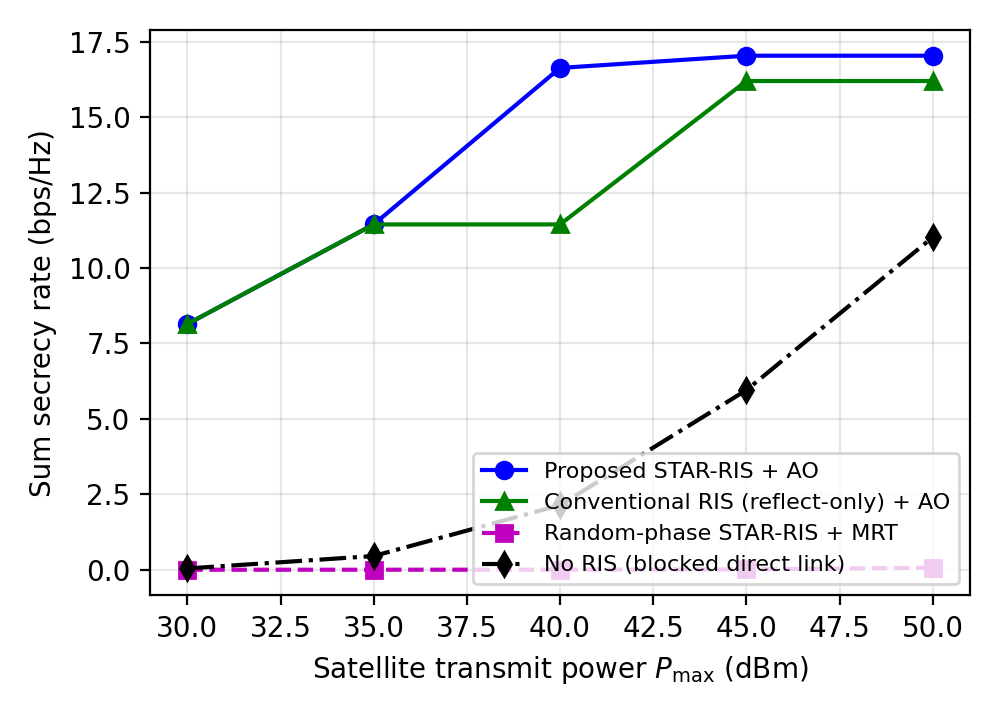
\includegraphics[width=\columnwidth]{figs/fig_secrecy_vs_pmax.png}
\caption{Sum secrecy rate vs.\ satellite transmit power: proposed STAR-RIS near-field ISAC vs.\ benchmarks.}
\label{fig:secrecy}
\end{figure}

\begin{figure}[t]
\centering
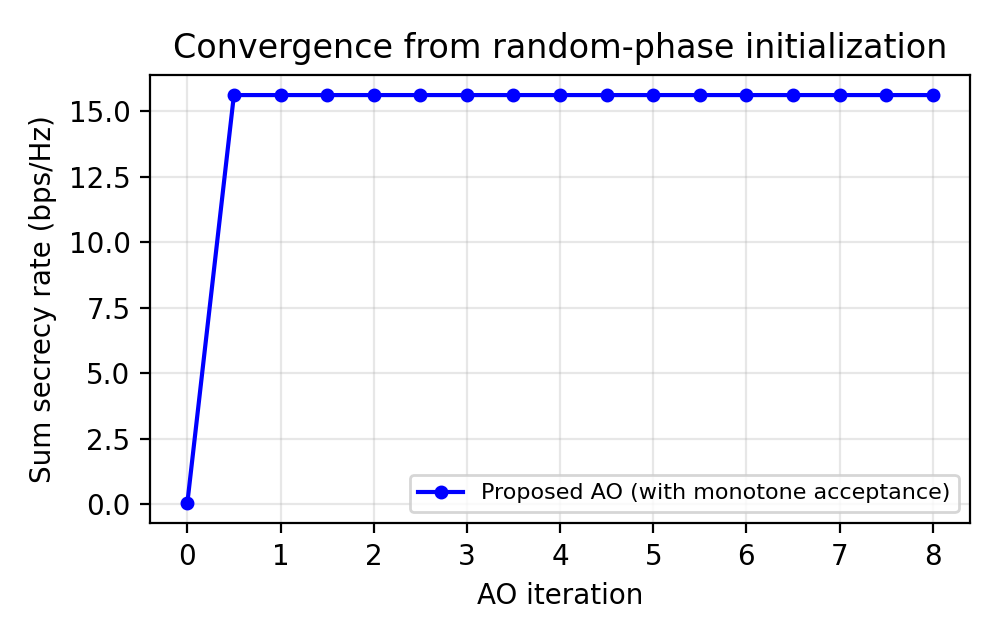
\includegraphics[width=\columnwidth]{figs/fig_convergence.png}
\caption{Convergence of the proposed AO algorithm ($P_{\max}=50$\,dBm).}
\label{fig:conv}
\end{figure}

\begin{figure}[t]
\centering
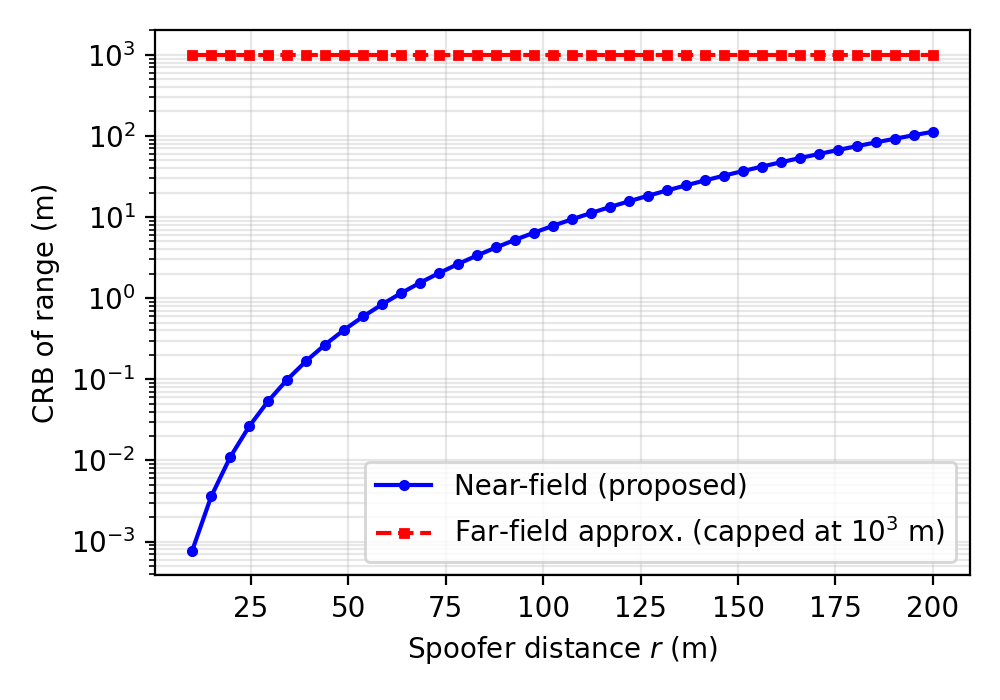
\includegraphics[width=\columnwidth]{figs/fig_crb.png}
\caption{CRB of the spoofer range estimate: near-field vs.\ far-field model.}
\label{fig:crb}
\end{figure}

\subsection{Robustness to Spoofer Localization Error}
Since the beamforming design relies on the spoofer channel \emph{reconstructed} from the sensed position (Remark~1), Fig.~\ref{fig:robust} evaluates the achieved sum secrecy rate when the true spoofer position deviates from the estimate by a random error of standard deviation $\sigma_e$ (60 Monte-Carlo realizations per level, fixed design). Two observations are made. First, at the accuracy actually delivered by the EKF ($\sigma_e \approx 0.36$\,m), the worst-case degradation over all realizations is only $4.5\%$ ($10.33$ vs.\ $10.81$\,bps/Hz), confirming that the ISAC sensing accuracy is sufficient for the secrecy design. Second, the mean achieved rate slightly \emph{increases} with $\sigma_e$: in this geometry the spoofer's nominal direction is nearly aligned with one user's near-field channel (the worst case, which the design suppresses at some rate sacrifice), so a position mismatch only decouples the spoofer from that user; the achieved rate never falls more than $4.5\%$ below the design value even at $\sigma_e=4$\,m, roughly seven times the array's transverse near-field resolution ($\approx 0.6$\,m at 40\,m).

\begin{figure}[t]
\centering
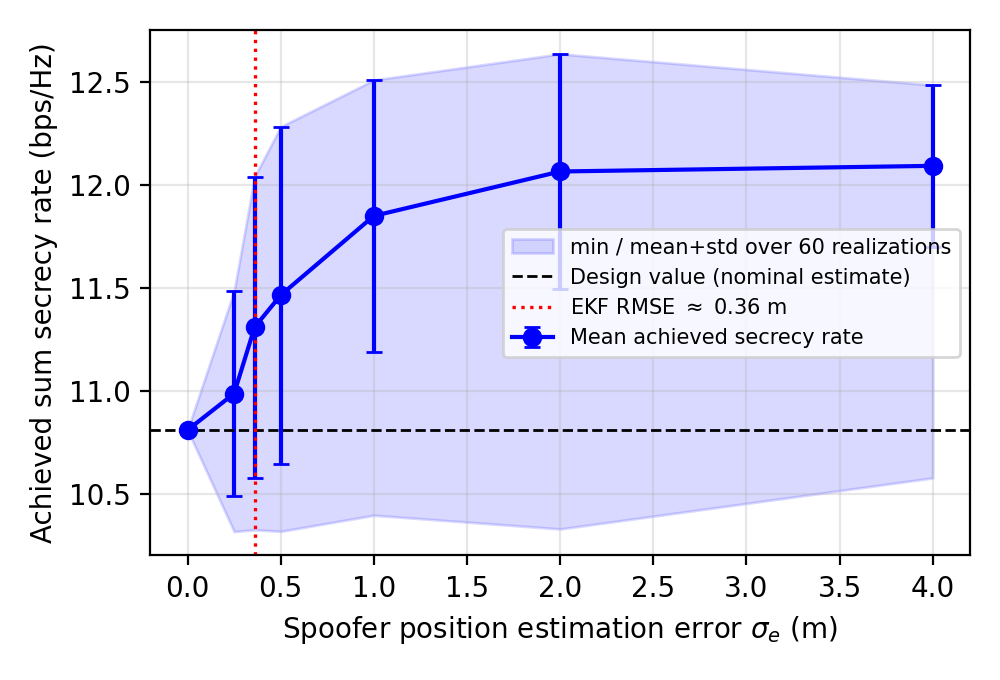
\includegraphics[width=\columnwidth]{figs/fig_robustness.png}
\caption{Achieved sum secrecy rate vs.\ spoofer-position estimation error (60 Monte-Carlo realizations; shaded: min to mean+std).}
\label{fig:robust}
\end{figure}

\begin{figure}[t]
\centering
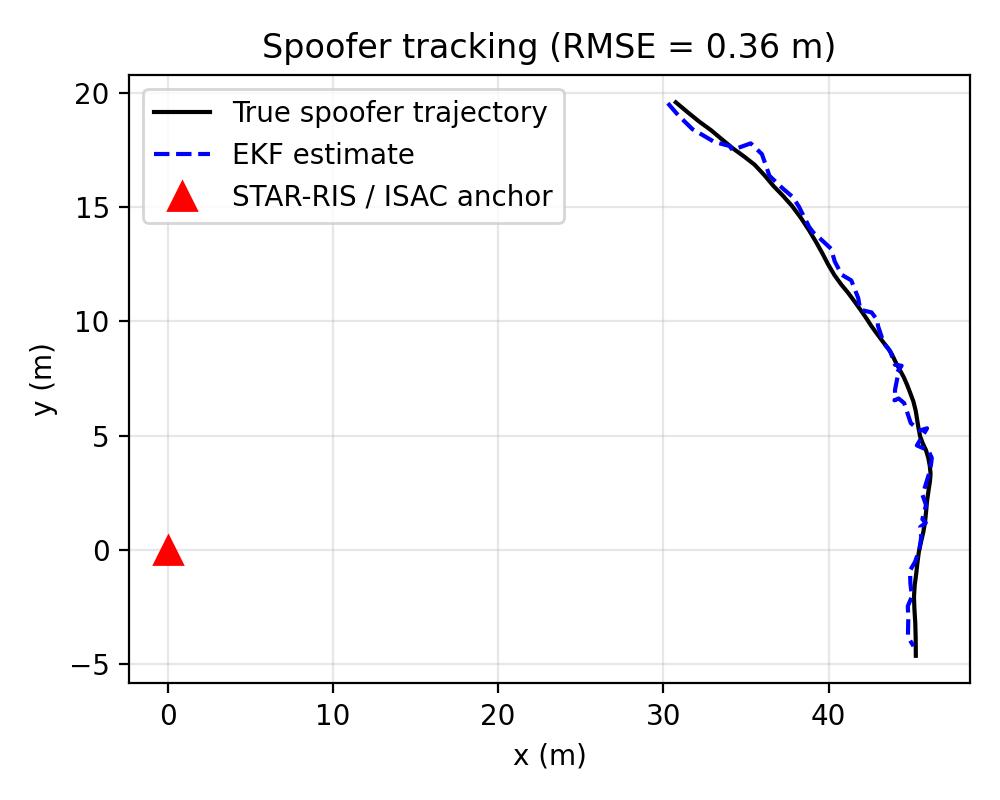
\includegraphics[width=\columnwidth]{figs/fig_ekf.png}
\caption{EKF-based spoofer trajectory tracking (position RMSE $\approx 0.36$\,m).}
\label{fig:ekf}
\end{figure}

\section{Conclusion}\label{sec:concl}

This work proposed a near-field secure ISAC framework with STAR-RIS for spoofing-resilient LEO satellite navigation. A hybrid far-field/near-field cascaded channel model with a Rician satellite link was developed, a joint satellite beamforming and STAR-RIS coefficient design was formulated with a CRB sensing constraint, and an AO/SCA-based algorithm was proposed. Numerical results confirmed that: (i) the proposed design consistently outperforms conventional RIS, random-phase STAR-RIS, and no-RIS benchmarks in sum secrecy rate; (ii) the algorithm converges within a few iterations; and (iii) near-field sensing enables spoofer range estimation that is fundamentally impossible under the far-field model; and (iv) the design degrades gracefully under spoofer-position estimation errors of the magnitude delivered by the EKF. Future work includes a dedicated anti-spoofing metric based on the user-level PNT error, an active-RIS benchmark and Monte-Carlo confidence intervals, the full CRB derivation over the cascaded channel, mobile users and multiple spoofers, AN covariance optimization, and hardware-impairment-aware designs.

The simulation code reproducing all figures is publicly available at \url{https://github.com/YOUR-USERNAME/leo-isac-starris}.


\bibliographystyle{IEEEtran}
\bibliography{references}

\end{document}
